\chapter{Introduction}
\section{Motivation}
    \label{sec:motivation}
    % Explain why the thesis is written. How will it contribute and what is the current status of things in the field.
    This master's thesis is a collaboration between the Innovative Immersive Technologies for Learning (IMTEL) VR lab an the Department of Geography, both at NTNU. The project is a continuation of the specialisation project \emph{Immersive Virtual Field Trip for Field Course in Physical Geography}\cite{specialisation}.
    
    Field trips are an important part of many courses, especially those surrounding nature. They do however carry many limitations and are generally costly and time intensive to perform. \emph{Virtual Field Trips} can help to get the most out of the field trips, especially by aiding students to prepare. In future Virtual Field Trips might even replace certain field trips, or offer an alternative to people who are hindered from attending.
    
    The field trip in question is for the course \emph{GEOG - 2012 Field Course in Physical Geography} at NTNU. The course is an introduction to the field, teaching students about different land formations and concepts, and how they are created\cite{geog2012}. The field trip is a two-hour drive from Trondheim and lasts from a Monday morning to Wednesday afternoon. During this period the students spend about 10 hours in the field in addition to a separate excursion on the Tuesday. A lot of preparation is needed both before and during the field trip, and there are expenses related to transporting and housing the students.
    
    There already exist several Virtual Field Trips, like Google Expeditions\cite{google_expeditions} where an educator can guide others through images. There are also applications using more advanced interaction, like the Climate Quest\cite{bachelor} application from NTNU where the user have to outrun a rising ocean level while shooting objects that are bad for the climate.
    %The new \emph{Oppdal Application} will, like Climate Quest, trading scalability for immersion. It will however focus on more on providing an opportunity to explore and learn, instead of invoking feelings around a topic.
    The  Virtual Field Trips will be combined with the advanced interaction to create a new application, named \textbf{The \ApplicationName}. This application will, like Climate Quest, trade scalability for immersion. It will however focus on more on providing an opportunity to explore and learn, instead of invoking feelings around a topic. The \ApplicationName \hspace{0.1cm} will be developed using \emph{Open Source} resources, meaning they will be available free of charge.
    
    As there already are Virtual Field Trip applications, there is also existing research on the subject. One of the leading sources of the research is Penn State University. From a news article at Hypergrid Business\cite{hypergrid} the research is summarised as collecting data on both real and virtual field trips, concluding that students are very positive the Virtual Field Trips. In an article from Penn State in 2017, Klippel and others\cite{developing_and_evaluating} evaluated the current development of VR field trips. They found that many earlier barriers had been overcome and that VR technology was ready to become more prominent in the market, something it arguably was and is still doing. Their research is however centred around simplistic Virtual Field Trips where interaction mostly is limited to looking around. The focus of this master's thesis is therefore around applications with more game-like interaction.
    
\section{Stakeholders and Target Audience}
    

\section{Research Questions}
    % Can iVFT contribute to better learning for a course with field trip?
    The research of this project will be centred around developing and testing the new \ApplicationName. LiDAR, a type of laser scanning, will be used to recreate a topological model of the area. Stereoscopic 360 images will be included to show the actual landscape and gameplay elements will be included to motivate and educate the users. The \ApplicationName \hspace{0.1cm}will be compared to a simpler, more scaleable application supplied by Penn State university, using the same images. The research questions of this master's thesis are:
    
    \SPACE
    
    \begin{itemize}
        \item \textbf{R1 - } \emph{Can a Virtual Field Trip be valuable as a support tool for courses with field trips?}
        
        Contributing to the current research on the field, the goal is to investigate how useful a Virtual Field Trip can be as a supportive learning tool to a university course.
        
        \SPACE
        
        \item \textbf{R2 - } \emph{Can the use of gameplay interaction elements in a Virtual Field Trip lead to a better learning outcome and than applications based on displaying images?}
        
        Expanding on the current research on the field, this will focus on comparing an application with little interaction, to one with more to see if there are differences in how well they work.
        
        \SPACE
        
        \item \textbf{R3 - } \emph{What game design theories apply and should be used in a Virtual Field Trip application?}
        
        As the goal is to investigate if a more interactive application can provide a better learning outcome, it is important to chose the right kind of interactivity. This will be done by reading appropriate literature to determine which elements that best improve the experience. 
        
        \SPACE
        
        \item \textbf{R4 - } \emph{How can a Virtual Field Trip be developed?}
        
        What are the tools and methods required for developing a Virtual Field Trip? Is it possible to automate parts of the process?
        
        \SPACE
        
        \item \textbf{R5 - } \emph{How does an omnidirectional treadmill compare to other ways of movement in VR?}
        
        What are the pros and cons of this input, especially for VR sickness and spatial awareness?
    \end{itemize}
    
    \todo{Merge R2 and R3?}
    
    \todo{Is R5 out of scope? Can it be commented on using only observation and 2-3 extra questions in questionnaire, or does it require a completely different test setup?}
    
    \todo{More focus on engagement than learning outcome}

\section{Research Method}
    % Create two applications and test them, use interviews with domain experts, and interviews and questionnaires with students that will take the course (and have taken it?).
    % Use development method with quantitative and qualitative evaluation
    Oates'\cite{research} Model of the Research Process is used to describe how this master's thesis is conducted. Simplified, Oates' model describes the research process divided into seven main parts, as seen in \cref{fig:oates}:
    
    \FloatBarrier
    \begin{figure}
        \centering
        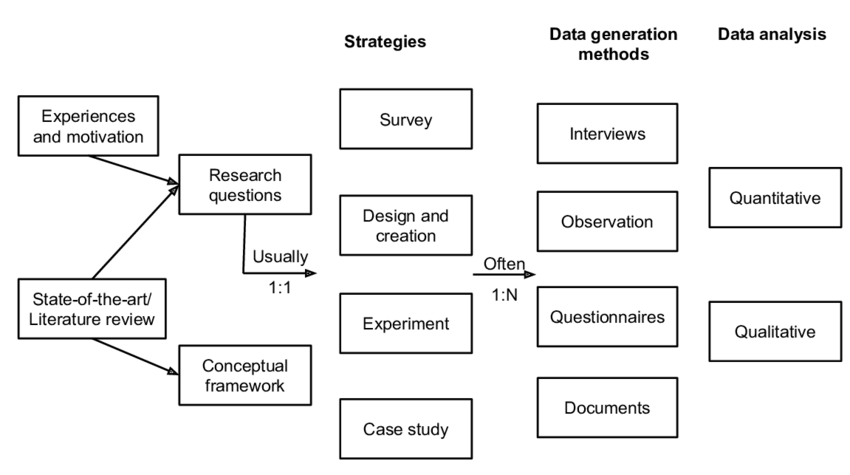
\includegraphics[width=\ImageWidth]{figures/oates.png}
        \caption{Oates' Model of the Research Process}
        \label{fig:oates}
    \end{figure}
    \FloatBarrier
    
    \todo{Highlight the used parst of oates' model}
    
    The four first parts of the research process are stated to be more or less the same for all types of research. These are the four ''boxes'' to the left of \cref{fig:oates}: Experiences and motivation, Research questions, State-of-the-art/Literature review and Conceptual framework. The personal experience and motivation combined with a literature review create the research questions. The literature review also leads to the conceptual framework that \emph{''makes explicit how you structure your thinking about your research topic and the process undertaken''}. The remaining three categories have elements that can differ depending on the type of research. As indicated in the figure, one research question typically leads to one strategy, whereas a strategy can lead to several methods of data generation.
    
    \SPACE
    
    \subsection*{Research Method of this Master's Thesis}
    This master's thesis conforms with Oates' model, with the four first parts present. This means that the project starts with existing experiences and motivation from the author. Combined with the literature review of the topic, research questions can be made. Additionally the conceptual framework of the terminology and relations take form and will be present throughout the thesis. The \textbf{Design and Create} strategy will be used to answer all of the presented research questions. This is done by implementing the application, allowing it to be tested and compared to other applications. Three data generation methods arise from the strategy: \textbf{Interviews}, \textbf{Observation} and \textbf{Questionnaires}. Students of the relevant course and domain experts will be invited to test the application. During these tests the users will be observed, then answer questionnaires and/or interviews. Finally, the data analysis approach will be both \textbf{Qualitative} and \textbf{Quantitative}. The Questionnaires will be the main data source for the quantitative data analysis, whereas the interviews and observations will supply data for the qualitative data analysis.

\section{Data handling}
    \todo{Write about data handling (GDPR) when running user tests}
